\section{Methodology}
\label{sec:meth}


We study all PE malwares submitted in November of 2015. 
In this section, we will firstly discuss how we collect data, 
and then we will present the general characteristics we observe.

\subsection{Data collection}

\begin{table}[h!]
\centering
\footnotesize
{
%\begin{tabular}{@{\hspace{3pt}}l@{\hspace{3pt}}|@{\hspace{3pt}}c@{\hspace{3pt}}}
\begin{tabular}{l|l}
\hline
Metadata Fields & Explanation \\
\hline                            
%\cline{1-1}
{\bf name}      & file name of the submitted sample \\
{\bf timestamp} & timestamp when the submission is conducted \\
{\bf source\_country} & the country where the submission is conducted \\
{\bf source\_id} & user id who conducts the submission\\
{\bf tags} & VirusTotal tag \\
{\bf link} & where to download the submitted sample \\
{\bf size} & file size \\
{\bf type} & file type \\
{\bf first\_seen} & when the same sample was first submitted \\
{\bf last\_seen} & when the same sample was last submitted \\
{\bf hashes} & including sha1, sha256, vhash, md5, and ssdeep\\
{\bf total} & how many engines analyze the sample\\
{\bf positives} & how many engines identify the sample as malicious \\
{\bf positives\_delta} & changes about {\bf positives} fields \\
{\bf report} & detailed detection report from each AV engine \\
%\multicolumn{2}{|l|}
\hline

\end{tabular}
}
\caption{Metadata fields of each submission got from VirusTotal private API.}
\label{tab:fields}
\end{table}

We download submission reports' metadata through private API of VirusTotal.
Table~\ref{tab:fields} shows all metadata fields.
For one report, if its tag field contains either ``peexe'' or ``pedll'', 
we consider the report is about a PE file. 
It is possible that VirusTotal private API returns redundant reports, 
and we use the combination of md5 and timestamp to detect and merge redundant reports.
We only rely on Microsoft antivirus engine to judge whether a submission is malicious or not, 
and which malware family the submitted malware belongs to. 
In total, we collect 43308091 reports and 4732502 PE malwares submitted
in November of 2015. 
The numbers of reports and malwares submitted each day are shown in Figure~\ref{fig:subnum}.

\textit{\underline{Threats to Validity.}}
Similar to all previous empirical study works, all our findings, experimental results, 
and conclusions need to be considered with our methodology in mind. 

VirusTotal private API only tracks which submission reports are sent to each downloader approximately, 
and there is no guarantee that all submission reports on VirusTotal can be downloaded successfully. 
It could be possible that we miss some malwares submitted to VirusTotal. 
We simply leverage Microsoft antivirus engine to decide whether one submission is malicious or not, 
and it is possible that Microsoft antivirus engine cannot make this decision precisely. 
However, how to get a precise label for a PE file is out of scope of this paper.  
Although there are huge mount of malwares on VirusTotal, we do believe that there are malwares never submitted to VirusTotal, 
and there are malwares submitted much later than when they appear in the real world.
However, there are no conceivable ways to study these malwares. 
We believe that malwares in our study provide a representative malware sample of the real world. 

\subsection{General characteristics}

We observe three characteristics after analyzing data we collect:

{\bf Observation 1:} 
most malwares are submitted only once to VirusTotal. 
We have collected 4732502 PE malware submissions, and there are in total 4038647 distinct PE malwares. 
On average, each PE malware is submitted 1.17 times to VirusTotal. 
We believe that most malwares are encountered by more than one VirusTotal user. 
We think this observation is likely to be caused by the fact that VirusTotal users 
tend to check whether their samples have already been submitted, 
before conducting their submissions, 
and the number of submissions is not a good indicator for malware popularity. 


{\bf Observation 2:} 
100 - 400 new malware families would appear each day. 
Figure~\ref{fig:new} shows new malwares appeared in November of 2015. 
We do not have any data before Nov. 1st, 
so there are much more new malware families in the first few days.
After that, the number of new malware families is roughly from 100 to 400. 
In total, there are 11311 malware families. 




\begin{figure}[t!]
\begin{center}
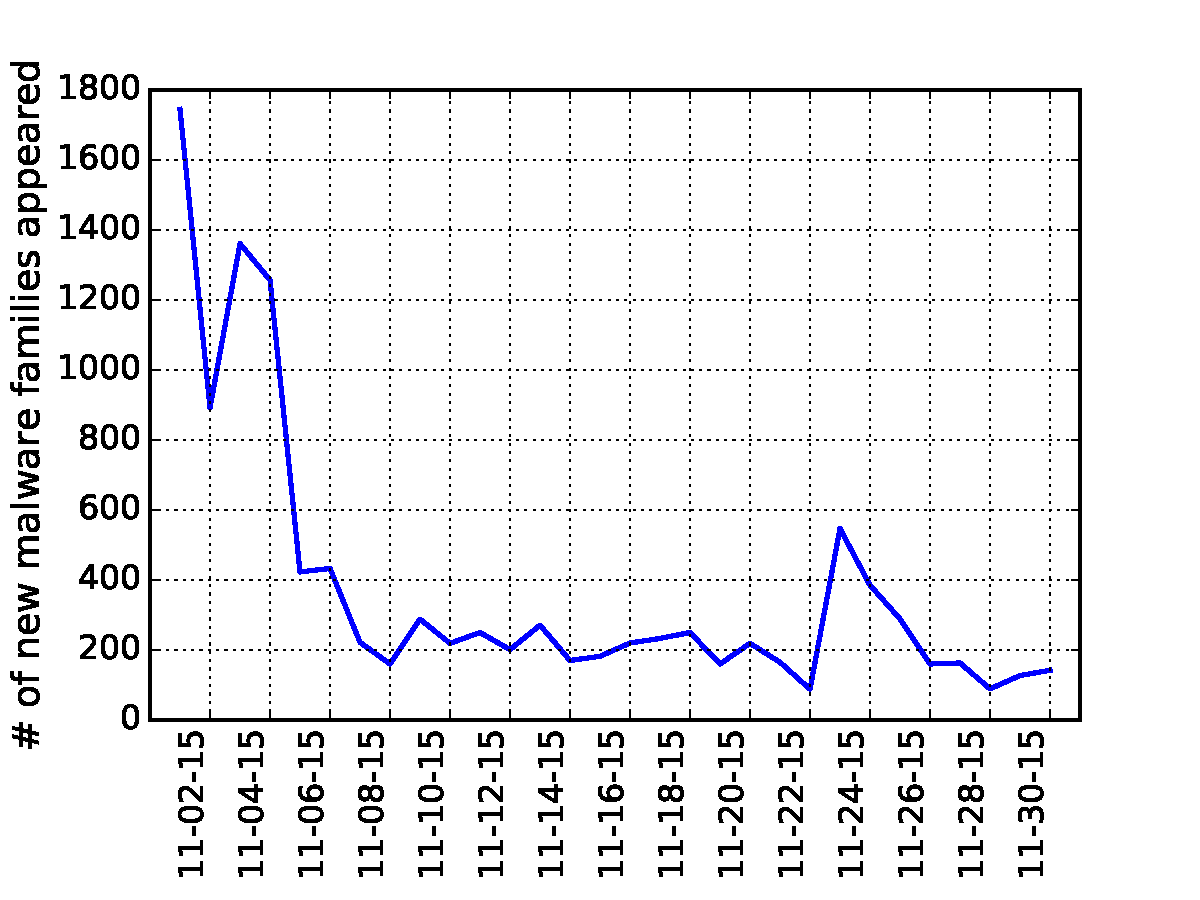
\includegraphics[width=3.0in]{figure/new_family}
\caption{The number of new malware families we observed each day in November of 2015.}
\label{fig:new}
\end{center}
\end{figure}

\begin{figure}[t!]
\begin{center}
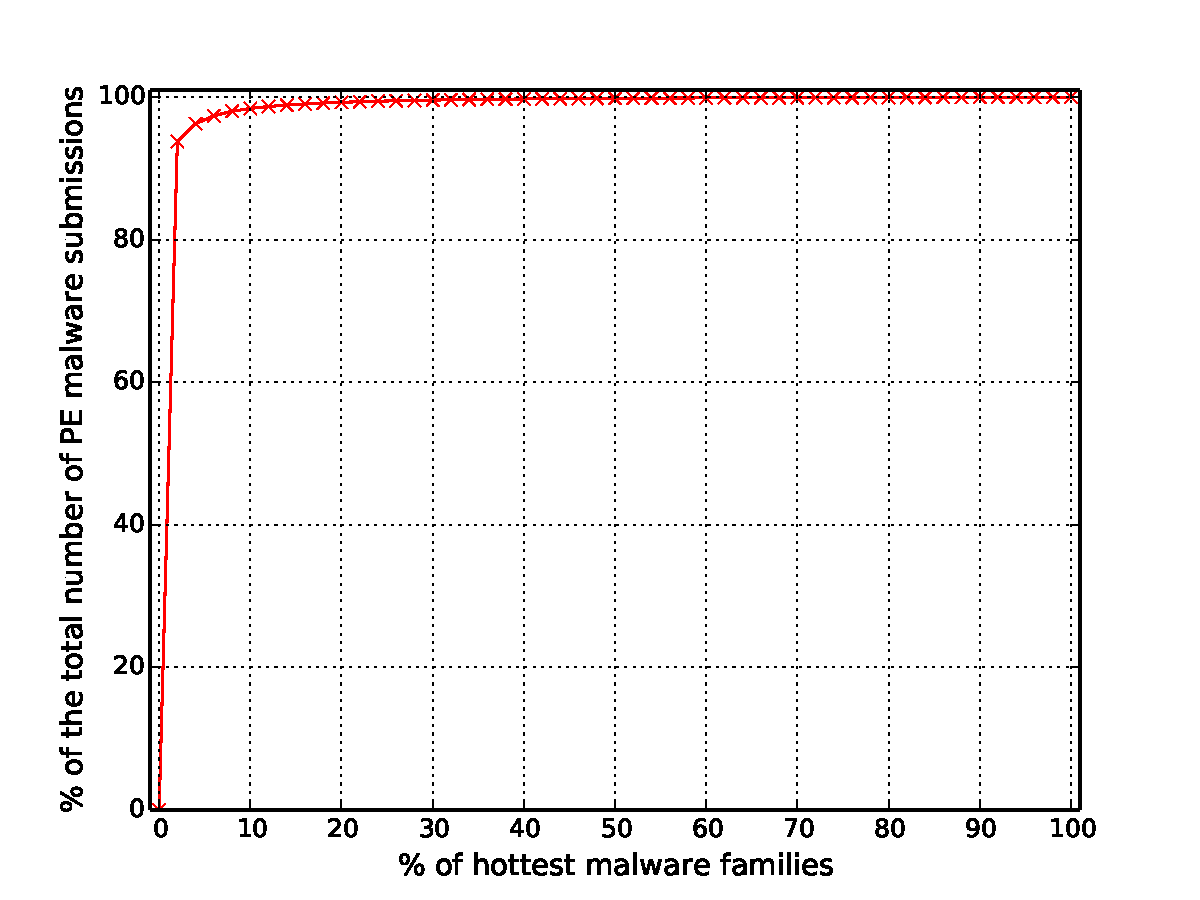
\includegraphics[width=3.0in]{figure/cum}
\caption{Skewness of malware families appearing in November of 2015.}
\label{fig:acum}
\end{center}
\end{figure}

{\bf Observation 3:} 
The distribution of malware families are highly skewed. 
As shown in Figure~\ref{fig:acum}, only small number of malware families are hot.
The distribution of malware families follows the well-known Pareto principle, 
and more than 90\% malware families take place in only 10\% malwares. 
The skewness of malware family distribution suggests that we could conduct effective hot malware family mining. 